


\subsection{Architecture}
For the implementation of the client application, \textit{React.js} which aims to solve the challenges involved when developing Web application with complex user interfaces, is applied. To have a better concept of how Graphicuss's client application is implemented, an overview of the file structure is listed in the figure \ref{fig:client-file-structure-imp}.

\subsubsection{Project Structure}
\begin{figure}[!htbp]
\centering
\begin{forest}
  for tree={
    font=\ttfamily,
    grow'=0,
    child anchor=west,
    parent anchor=south,
    anchor=west,
    calign=first,
    edge path={
      \noexpand\path [draw, \forestoption{edge}]
      (!u.south west) +(7.5pt,0) |- node[fill,inner sep=1.25pt] {} (.child anchor)\forestoption{edge label};
    },
    before typesetting nodes={
      if n=1
        {insert before={[,phantom]}}
        {}
    },
    fit=band,
    before computing xy={l=15pt},
  }
[client
  [components/
    [AppBar/
      [index.js]
      [style.css]
    ]
    [...]
  ]
  [containers/]
  [models/]
  [utils/]
  [index.js]
  [index.html]
  [...]
]
\end{forest}
\caption{Overview of client app's file structure}
\label{fig:client-file-structure-imp}
\end{figure}

\begin{itemize}
  \item 
  \textbf{components/}: all components are defined by extending basic \textit{React.Compoent}. Each custom component has an \textit{index.js}, which processes the logics of view rendering and applies view models to the template. \textit{style.css} defines the CSS style of the HTML DOMs within a component.
  \item 
  \textbf{containers/}: containers are compositions of components.
  \item 
  \textbf{models/}: in model directory, data models for the components are defined. In addition, the definition of APIs and processing after data acquisition  also take place here.
  \item 
  \textbf{index.js \& index.html}: \textit{index.js} is the entry point of the app, which will instantiate the React instance and render the views into a specific DOM defined  in \textit{index.html}
\end{itemize}


\subsubsection{Achitecture of Client}

An overview of the client application's architecture is revealed in figure \ref{fig:client-arch-imp}. 

\begin{figure}[!htbp]
  \centering
    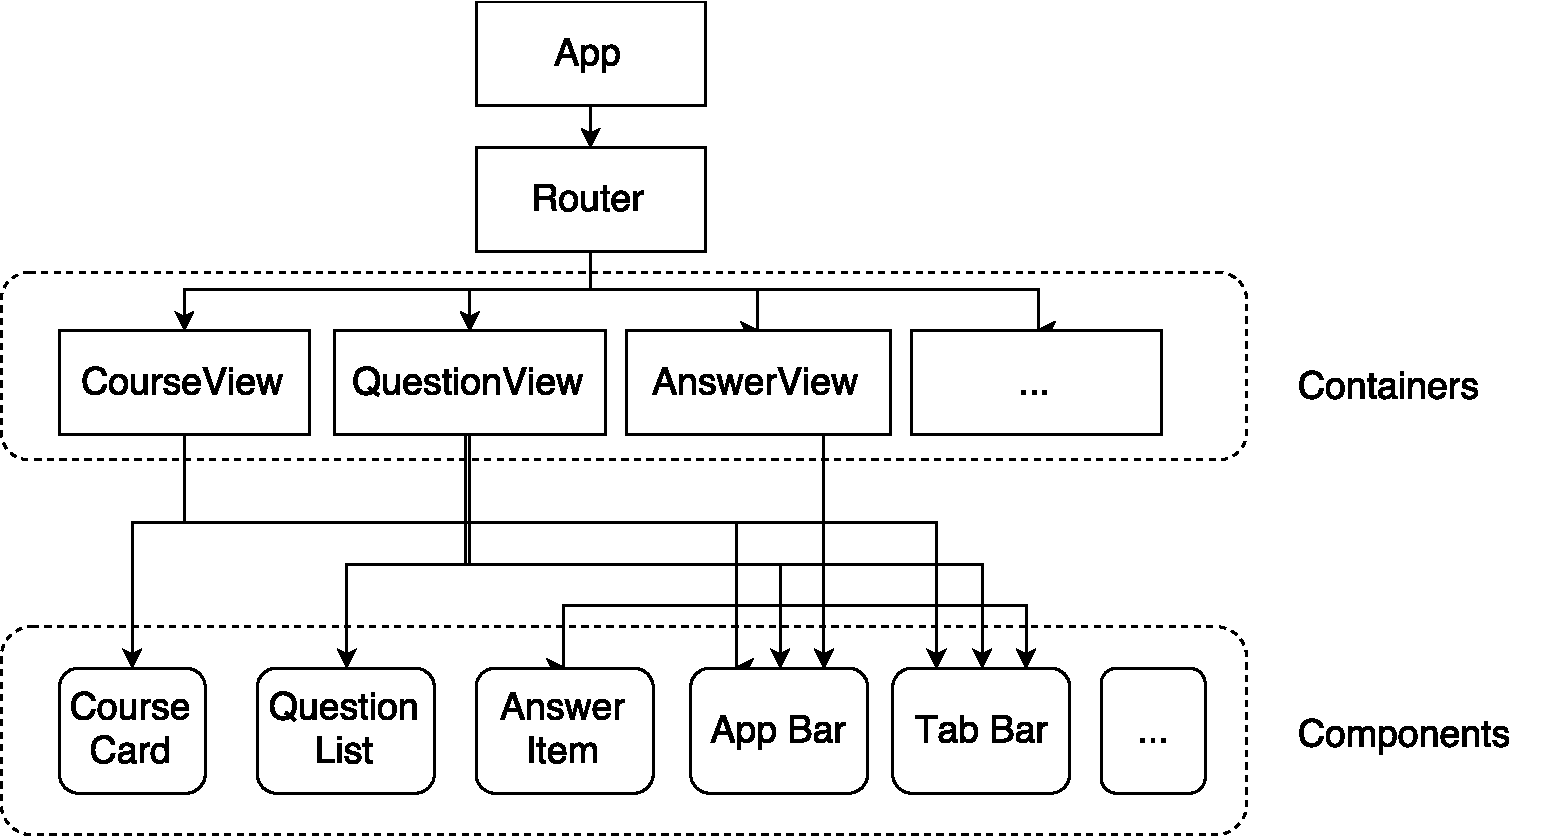
\includegraphics[width=1\textwidth]{Figures/imp-client-arch.pdf}
  \caption{Overview of client architecture}
  \label{fig:client-arch-imp}
\end{figure}
% client arch, App -> router containes rotes -> different container -> components(Compisition... for containers!) xuxian for layer (App, router, container, components)

In the React application, \textit{Router} is also regarded  as a component, in which different matching rules of the URL are defined. If the URL requested by the user is matched, a correlate view will be rendered according to the definition of routes. Code list \ref{list:router-client-imp} shows the implementation of defining a \textit{Router} component.

\begin{lstlisting}[language=HTML, caption=Router in client app , label={list:router-client-imp}]
<Router history={history}>
  <Route path="/" component={App}>
    <Route path="auth" component={AuthView} />
    <Route path="courses" component={CoursesView} />
    <Route path="courses/:courseId" component={QuestionsView} />
    <Route path="questions/:questionId" component={AnswersView} />
  </Route>
</Router>
\end{lstlisting}

Containers such like \textit{CourseView}, \textit{QuestionsView} or \textit{AnswersView} are compositions of components in fact. The way how component acquires view model is that the parent component passes values to its child component by defining the properties of the child component. So the data flow starts from the root component and goes through every child component. 

How to manage the data flow and control the rendering behavior will be discussed later in the sub section \ref{subsection:data-flow-react-imp}.


\subsection{Composition of Components}

\subsubsection{React Component}

Defining a new \textit{Component} with React.js must extend the \textit{React.Component} class and implement the \textit{render()} function, which will be called when the component is instantiated. Afterwards, the template as well as the composition of components are rendered to plain HTML.  A simplified example of building a \textit{CourseView} component is represented in code list \ref{list:course-view-render-imp}.

\begin{lstlisting}[language=HTML, caption=Rendering \textit{CourseView} with multiple \textit{CourseCard} components , label={list:course-view-render-imp}]
class CoursesView extends React.Component {
  render() {
    const courses = this.props.courses
    return (
      <div>
        {
          courses.map( (course) =>
            <CourseCard course={course} key={course._id}></CourseCard>
          )
        }
      </div>
    ); 
  }
}
\end{lstlisting}

As mentioned above, the parent components pass data through as the properties of child components. Within the \textit{CoursesView}, \textit{courses} could be read from its properties which is defined while \textit{CourseView} is composed. In the \textit{render()} function of \textit{CourseView}, \textit{courses} are traversed and each single \textit{course} will be passed into the \textit{CourseCard} as its property. Which means, as \textit{CourseView} is rendered, all \textit{CourseCard} components within it will also call their own \textit{render()} functions with the data model passed in. Data flows from top to bottom, likewise, views are rendered from parent to child components.

\subsubsection{Composition}
\textit{Components} are the core of React. All each view and its view model of the client application is represented as a React \text{Component}. And the whole client app is actually a composition of React components. An example of \textit{CoursesView} is taken in figure \ref{fig:course-view-composition-imp}.

\begin{figure}[!htbp]
  \centering
    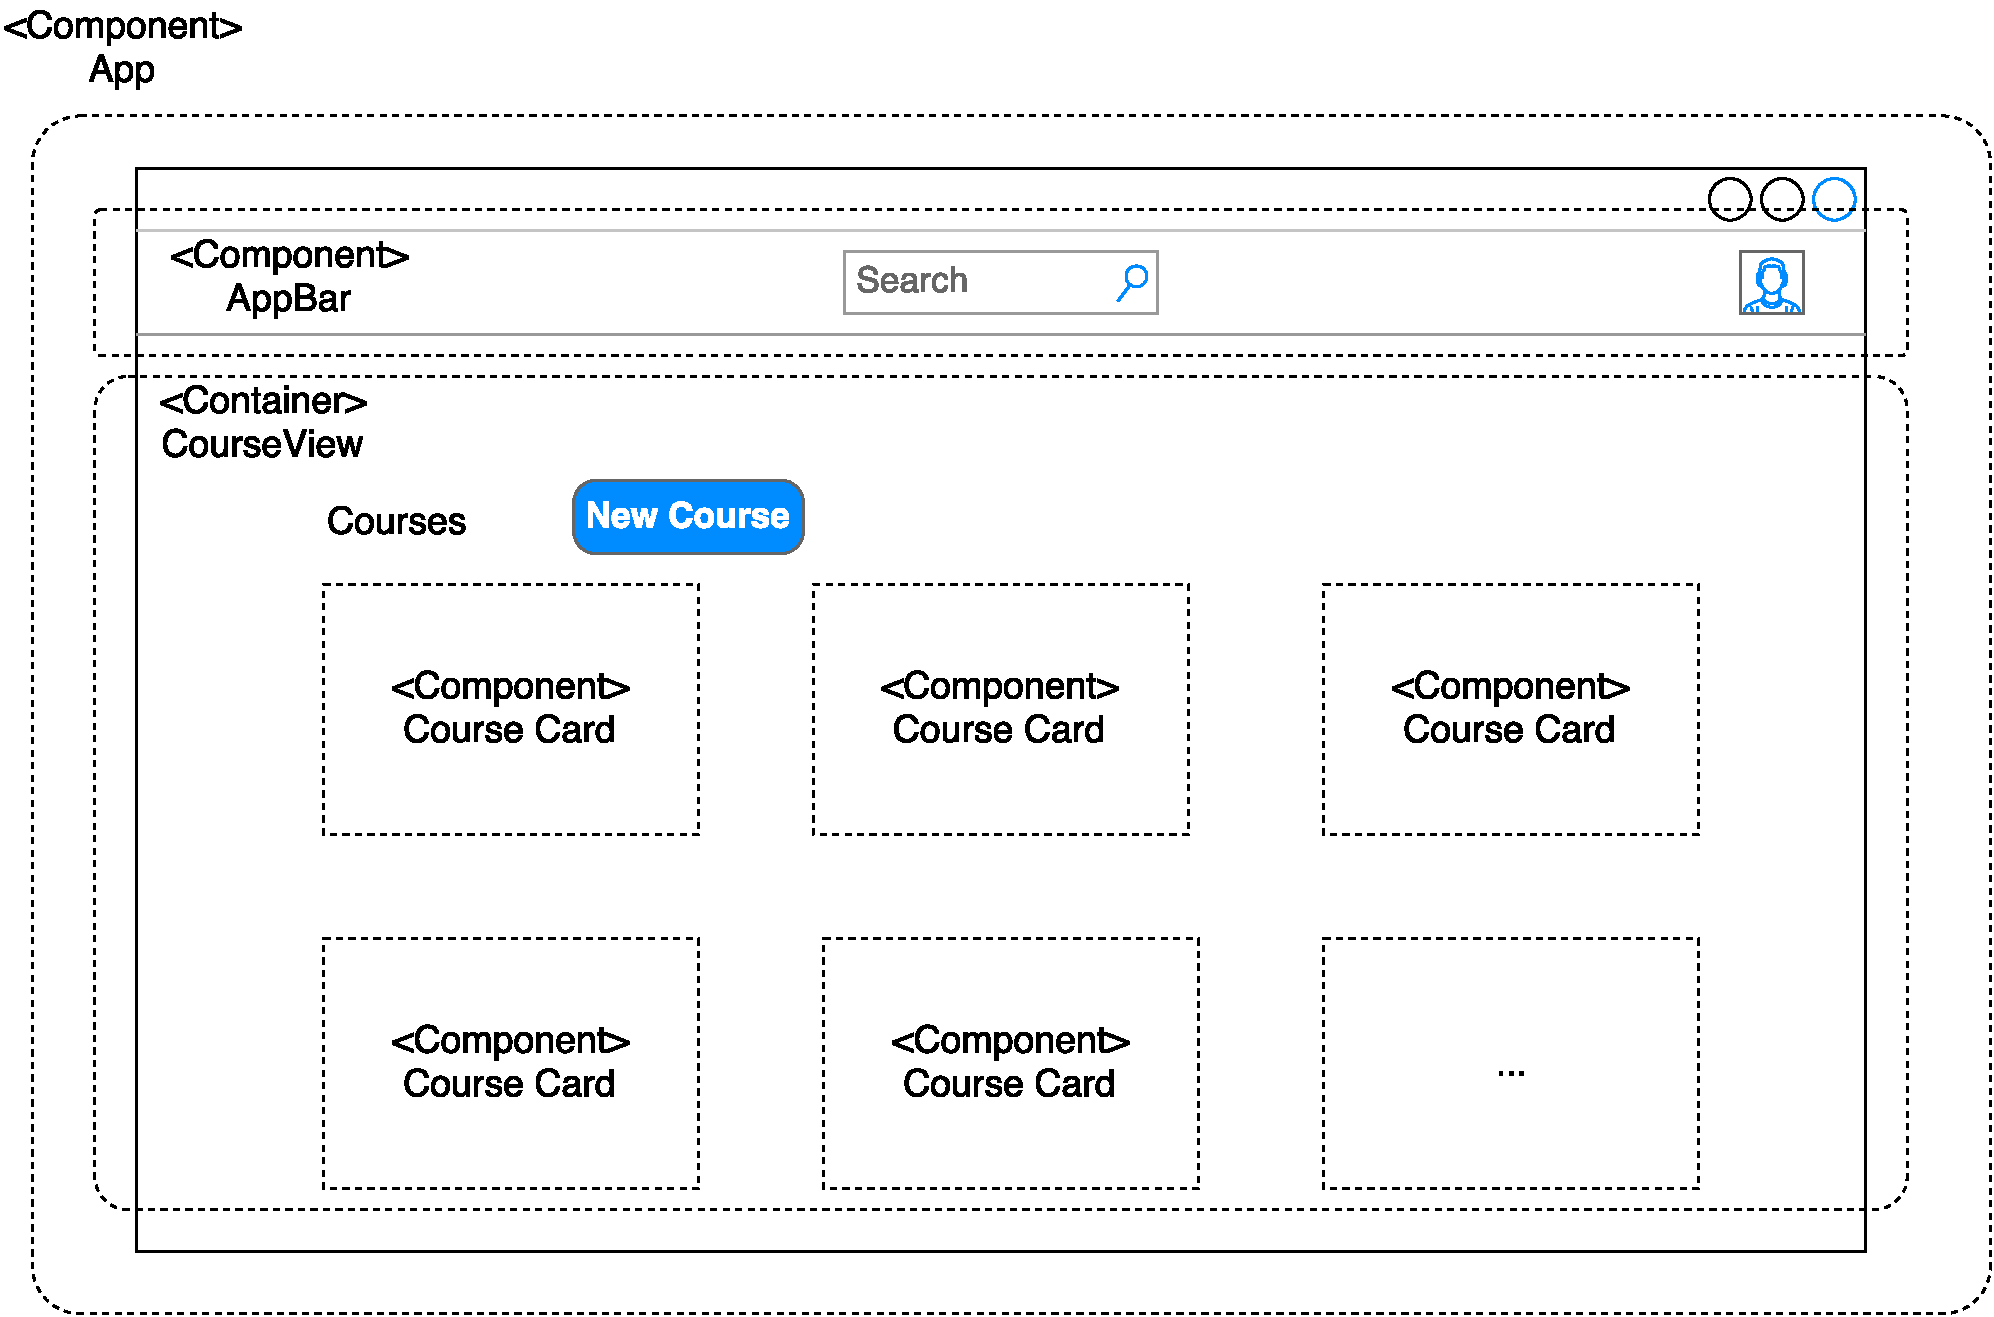
\includegraphics[width=1\textwidth]{Figures/imp-course-view-composition.pdf}
  \caption{Composition of components in courses' page}
  \label{fig:course-view-composition-imp}
\end{figure}
% Course Page. Composition, App bar, tab view, course page, course card ...

At the top of the view is a component called \textit{AppBar}, which is also composed with another component \textit{SearchBox}. \textit{ContentSection} is a container for the main content, which will be replaced and re-rendered if the context of router changes. In this example, the route \textit{/courses} is applied, and the component \textit{CourseView} is rendered into \textit{ContentSection}. 

\textit{CourseView} is also a composition of components: a list of \textit{CourseCard} components and also other components such as submit button component and popover component for creating new courses. 

In principle, building other views is the same approach. Composition of components constructs the all views. With fine-grained components, the client app becomes much extensible and maintainable.


\subsection{Data Flow}\label{subsection:data-flow-react-imp}

Since data is passed as properties of components from top to bottom in the React application, maintaining data models between components and the data flow through components is a problem. \textit{Flux}\footnote{http://facebook.github.io/flux/ - accessed 18 July 2016} is a architecture which aims to solve this problem. Data flows in a single direction, which keeps the process simple and ensures the correctness of view rendering.

There are four main concepts of Flux architecture: 
\begin{itemize}
  \item 
  \textbf{View}: view layer which references the data model and renders the data model into the template.
  \item 
  \textbf{Action}: action made by view, trigger for processing data model, for example a mouse click event.
  \item 
  \textbf{Dispatcher}: receives the actions and run callback functions to modify the data model.
  \item 
  \textbf{Store}: stores the states of data, if the states of data are changed, store will notify the views to re-render with the new state of data.
\end{itemize}

\begin{figure}[!htbp]
  \centering
    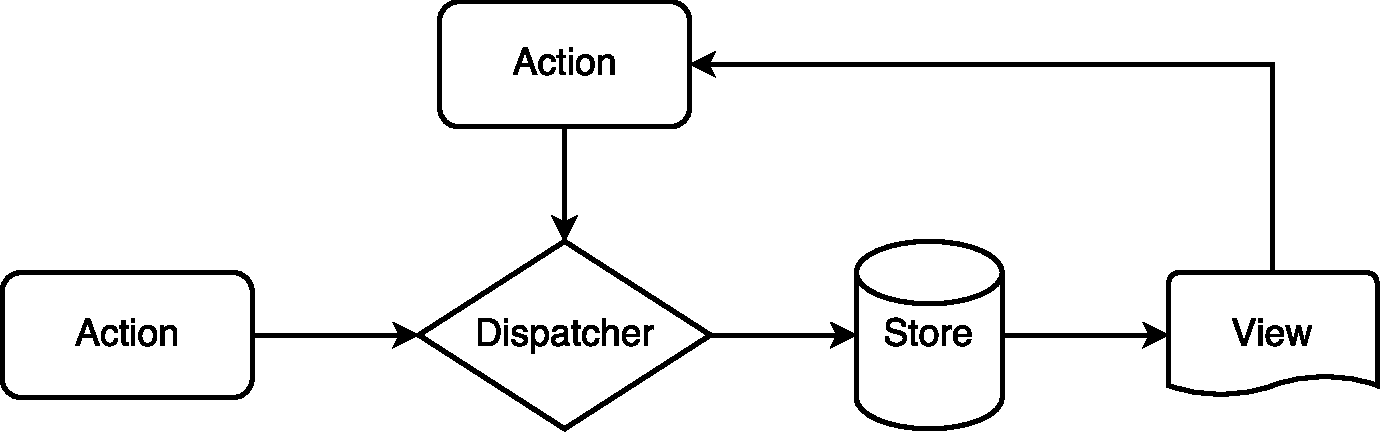
\includegraphics[width=0.9\textwidth]{Figures/imp-flux-arch.pdf}
  \caption{Data flow in Flux architecture}
  \label{fig:flux-arch-imp}
\end{figure}

The main process of data flow in Flux architecture is illustrated in figure \ref{fig:flux-arch-imp}. The key of Flux is unidirectional data flow. For example, a user wants to submit a new answer to a certain question in Graphicuss system, as soon as the new answer is synchronized with the server side, the new answer will be rendered into the answer list attached to the question. The process of data flow in this case is described as follows:
\begin{enumerate}
  \item 
  User submits a new answer, \textit{Action(NEW\_ANSWER)} is triggered.
  \item 
  \textit{Action} requests the API for submitting new answer.
  \item 
  \textit{Dispatcher} receives the \textit{Action(NEW\_ANSWER)} and inserts an entry of this new answer into the \textit{answers} state which is stored in \textit{Store}.
  \item 
  Since the state of \textit{answers} is changed, \textit{Store} starts notifying the views to re-render.
  \item 
  Views re-render the templates with the new state of \textit{answers} which contains the new submission of answer.
\end{enumerate}


To validate the final result of the implementation on client side, screenshots for two representative views: \textit{CourseView} and \textit{QuestionsView} are taken in figure \ref{fig:ss-class} and \ref{fig:ss-question}. 

\begin{figure}[!htbp]
  \centering
    \frame{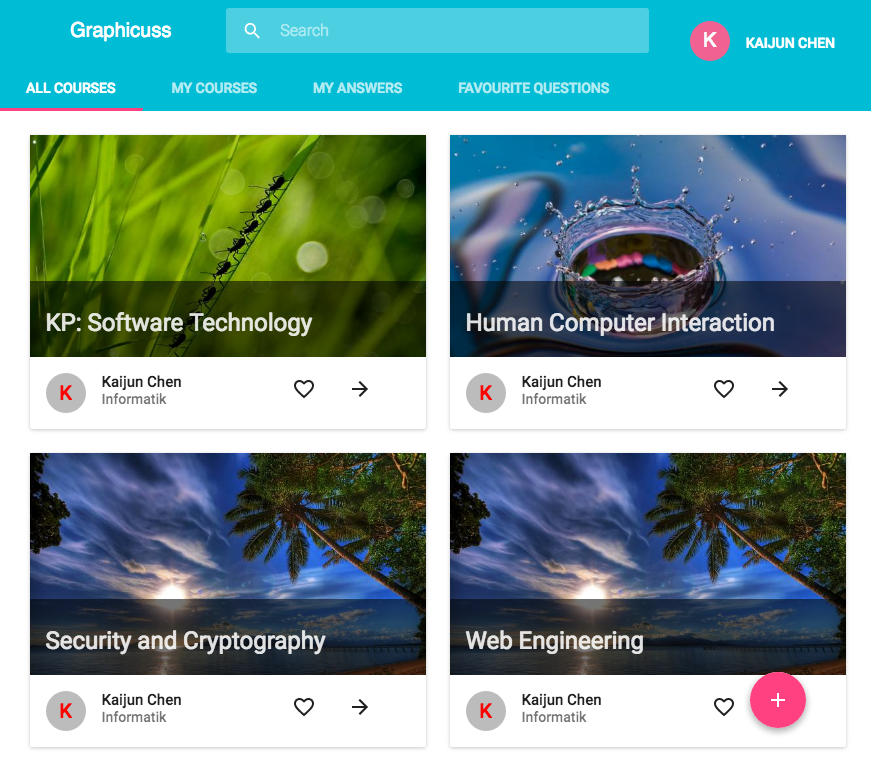
\includegraphics[width=0.9\textwidth]{Figures/ss-class.png}}
  \caption{Screenshot of course view}
  \label{fig:ss-class}
\end{figure}
\begin{figure}[!htbp]
  \centering
    \frame{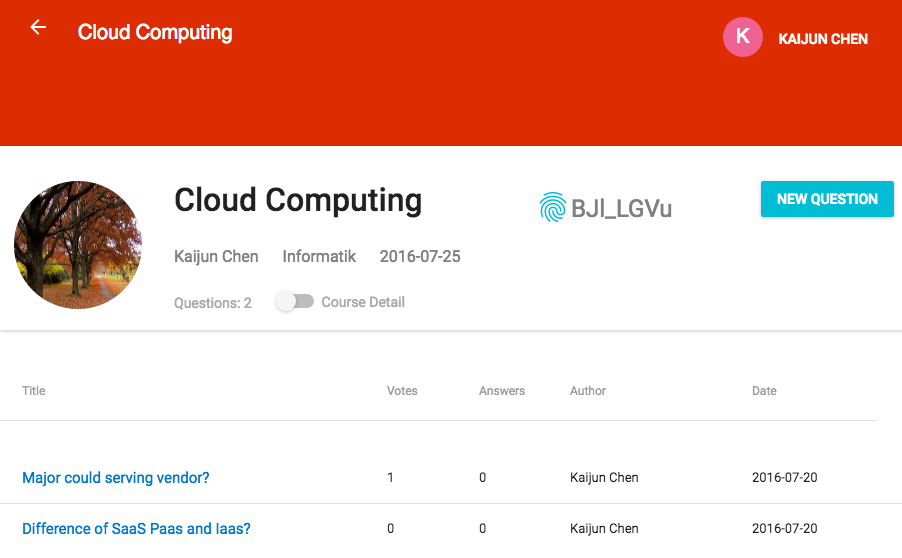
\includegraphics[width=0.9\textwidth]{Figures/ss-question.png}}
  \caption{Screenshot of questions view within a class}
  \label{fig:ss-question}
\end{figure}